\section{Results}
\label{sec:results}

\subsection{Cortical Planning and Counterfactual Critique (\op{v1} $\to$ \op{v2} $\to$ \op{v3-Pro})}
\label{sec:res_beat}

Table~\ref{tab:planner_critic} and Figure~\ref{fig:training} (left, centre) evaluate architectural and objective scaling across \op{Cortex} and \op{Cingulate}. Moving from uniform regression (\op{v1}) to sharp-cut and accompaniment-floor regularisation (\op{v2}) cut held-out bar timing error by $25\%$ ($0.429 \to 0.320$ bars) and lifted zero-shot recipe agreement on human-audited \op{owner.jsonl} to $86.14\%$ ($87/101$). Scaling to \textbf{Cortex v3-Pro} ($8\text{L}/192\text{D}$, $3.60$\,M params, $20{,}000$ steps with beat-loudness jitter) halves held-out timing error again on the strictly unseen $5{,}707$-example \op{val.jsonl.gz} benchmark to $\mathbf{0.165}$\,\textbf{bars} ($96.77\%$ final / $98.63\%$ peak recipe accuracy, $\mathbf{0.0170}$ 8-lane fader MAE) while achieving $99.0\%$ ($100/101$, $0.05$\,bar MAE) preference alignment on \op{owner.jsonl} at $38.03$\,ms single-threaded CPU latency (FP32-vs-FP16 max deviation $0.00164$ bars).

Similarly, scaling \textbf{Cingulate v3} across the full $30$-defect taxonomy with $50\%$ on-GPU $7$-mode counterfactual synthesis reaches $\mathbf{97.28\%}$ (\op{v3-Base}, $8.71$\,ms) and $\mathbf{97.00\%}$ (\op{v3-Pro}, $16.66$\,ms) accuracy on unseen \op{val.jsonl.gz}, cutting false positives on \op{owner.jsonl} from $7$ (\op{v1}) and $5$ (\op{v2}) down to $\mathbf{0}$ on \op{v3-Base} ($\mathrm{TP}=91, \mathrm{FP}=0, \mathrm{TN}=41$, $\mathbf{100.0\%}$ precision) and $\mathbf{1}$ on \op{v3-Pro} ($\mathrm{TP}=94, \mathrm{FP}=1, \mathrm{TN}=40$, $98.9\%$ precision; $100$\,ms for Best-of-$6$ reranking).

\begin{table*}[t]
\centering
\caption{Progression of \textbf{Cortex} (planner) and \textbf{Cingulate} (conflict monitor) from uniform regression (\op{v1}) to sharp-cut alignment (\op{v2}) and scaled domain-randomized transformers (\op{v3-Base} / \op{v3-Pro}). Held-out \op{val.jsonl.gz} ($n=5{,}707$) is strictly unseen across all versions; \op{owner.jsonl} ($n=142$) is zero-shot held out in \op{v1/v2} and folded into preference alignment in \op{v3}$^\S$.}
\label{tab:planner_critic}
\footnotesize
\setlength{\tabcolsep}{4.0pt}
\resizebox{\linewidth}{!}{\begin{tabular}{@{}llcccccr@{}}
\toprule
Planner (\op{cortex.*}) & Architecture \& Objective & Held-out Rec.$\uparrow$ & Held-out Bars$\downarrow$ & Lane MAE$\downarrow$ & Owner Align.$\uparrow$ & FP16 $\Delta_{\max}$ & CPU 1-thr \\
\midrule
\op{Cortex v1} & $6\text{L}/128\text{D}$, uniform BCE + $L_1$ & $94.29\%$ & $0.429$ & $0.0470$ & $85.15\%$ (zero-shot) & $0.0049$ & $16.16$\,ms \\
\op{Cortex v2} & $6\text{L}/128\text{D}$, $+ 6\times \mathcal{L}_{\text{cut}} + \mathcal{L}_{\text{energy}}$ & $95.16\%$ & $0.320$ & $0.0312$ & $86.14\%$ (zero-shot) & $0.0052$ & $16.74$\,ms \\
\op{Cortex v3-Base} & $6\text{L}/128\text{D}$, $+ \text{dB jitter}, 20\text{k}$ steps & $96.89\%$ ($96.9\%$ pk) & $0.205$ & $0.0221$ & $99.0\%$ ($0.04$ bars)$^\S$ & $0.0029$ & $17.30$\,ms \\
\textbf{\op{Cortex v3-Pro}} & $\mathbf{8\text{L}/192\text{D}}$ ($3.60$\,M), $20\text{k}$ steps & $\mathbf{98.63\%}$ ($98.6\%$ pk) & $\mathbf{0.188}$ & $\mathbf{0.0173}$ & $\mathbf{99.0\%}$ ($\mathbf{0.05}$ \textbf{bars})$^\S$ & $\mathbf{0.0016}$ & $38.03$\,ms \\
\midrule
Monitor (\op{cingulate.*}) & Corruption Synthesis & Held-out Acc.$\uparrow$ & Defect Taxonomy & Neg.\ Ratio & Owner Prec.$\uparrow$ & FP16 $\Delta_{\max}$ & CPU 1-thr \\
\midrule
\op{Cingulate v1} & $4\text{L}/96\text{D}$, offline perturbations & $96.74\%$ & $11$ heads & $0\%$ GPU & $87.9\%$ (zero-shot) & $0.0012$ & $8.33$\,ms \\
\op{Cingulate v2} & $4\text{L}/96\text{D}$, $+ 35\%$ GPU hard negs & $97.39\%$ pk & $11$ heads & $35\%$ GPU & $89.4\%$ (zero-shot) & $0.0011$ & $8.84$\,ms \\
\op{Cingulate v3-Base} & $4\text{L}/96\text{D}$, 7-mode counterfactuals & $\mathbf{97.35\%}$ ($97.3\%$ pk) & $30$ heads & $50\%$ GPU & $\mathbf{100.0\%}$ ($\mathrm{FP}=0$)$^\S$ & $0.0053$ & $8.71$\,ms \\
\textbf{\op{Cingulate v3-Pro}} & $\mathbf{6\text{L}/128\text{D}}$ ($1.23$\,M), 7-mode CF & $\mathbf{96.81\%}$ & $\mathbf{30}$ \textbf{heads} & $\mathbf{50\%}$ \textbf{GPU} & $\mathbf{98.9\%}$ ($\mathrm{FP}=1$)$^\S$ & $0.0028$ & $16.66$\,ms \\
\bottomrule
\end{tabular}}
\end{table*}


\paragraph{Blind listening discovery and acoustic waveform verification.}
Table~\ref{tab:human_eval} and Figure~\ref{fig:ablation} document how blind listening guided our progression from \op{Rule} to \op{v3}:
\begin{enumerate}
  \item \textbf{Rule baseline ($6$ mixes):} Listener preferences tracked rule structural confidence ($0.45 \to$ ``excellent / great'' on half/double-time harmonic locks \op{0hkR93}$\leftrightarrow$\op{6wPupZ}; $0.18 \to$ ``fits, not quite a transition'' on \op{5ihq4q}$\to$\op{0I4cfb}, which \op{Cingulate} independently scored $\hat{q}=0.0002$ with \op{CutNotTransition} $=0.983$).
  \item \textbf{Eliminating $-33.6$\,dBFS pre-entry holes (\op{7yoqSl}$\to$\op{6N185A}):} \op{Cortex v1} hedged entry timing by ducking Deck~$A$ bass ($0.23$) and chords ($0.18$) $2.5$\,s before Deck~$B$ entered ($-33.64$\,dBFS trough; rejected in blind listening despite \op{Cingulate v1}'s false-positive $0.977$). Combining sharp-cut regularisation, accompaniment-floor constraints, and vocal-onset handoff in \op{v3} raised minimum blend loudness by $\mathbf{+10.55}$\,\textbf{dB} to $\mathbf{-23.09}$\,\textbf{dBFS} (\op{Cingulate} $0.996$, $0.0$\,ms beat drift).
  \item \textbf{Skipping $4.6$\,s silent vocal intros (\op{6wPupZ}$\to$\op{0hkR93}):} Whereas \op{v1} smeared Deck~$A$'s vocalist mid-word ($5/10$) and \op{v2} opened Deck~$B$ into $4.6$\,s of empty intro, Eq.~\eqref{eq:handoff} pinpointed sustained singing in \op{0hkR93} at $t_B = 4.94$\,s ($u_{\text{handoff}}=-3.0$), keeping Deck~$A$ singing at unity gain right into a breath-echo handoff over a $-2.5$\,dB chord pocket.
\end{enumerate}

\begin{table*}[t]
\centering
\caption{Iterative blind listening and acoustic waveform verification across Rule, Neural \op{v1}, Sharp-Cut \op{v2}, and Vocal-Onset-Locked \op{v3} mixes. $\min\mathrm{RMS}_{1\text{s}}$ measures the deepest 1\,s loudness trough inside the transition window.}
\label{tab:human_eval}
\footnotesize
\setlength{\tabcolsep}{3.6pt}
\resizebox{\linewidth}{!}{\begin{tabular}{@{}llllrrrl@{}}
\toprule
Gen.\ & Pair ($\mathrm{BPM}_A \to \mathrm{BPM}_B$, Key) & Recipe & $u_{\text{handoff}}$ & Cingulate & Drift & $\min\mathrm{RMS}_{1\text{s}}$ & Blind Human Verdict / Acoustic Outcome \\
\midrule
Rule & \op{0hkR93}$\to$\op{6wPupZ} ($78\!\to\!159$, 6A) & \op{VoiceOverBeat} & $-8.38$ & $0.990$ & $0.0$\,ms & $-25.8$\,dB & \textbf{``Excellent''} (highest rule confidence $0.45$) \\
Rule & \op{6wPupZ}$\to$\op{0hkR93} ($159\!\to\!78$, 6A) & \op{VoiceOverBeat} & $-6.00$ & -- & $0.0$\,ms & $-27.9$\,dB & \textbf{``Great''} (half-time 2:1 harmonic lock) \\
Rule & \op{5ihq4q}$\to$\op{0I4cfb} ($120\!\to\!119$, 8A/9A) & \op{Sneak} & $-8.00$ & $0.000$ & $0.0$\,ms & $-21.4$\,dB & ``Fits, not quite a transition'' (conf.\ $0.18$) \\
\midrule
\op{v1} & \op{7yoqSl}$\to$\op{6N185A} ($92\!\to\!91$, 6A) & \op{VoiceOverBeat} & $-16.25$ & $0.977^\dagger$ & $0.0$\,ms & $-33.64$\,dB & \textbf{Rejected:} 2.5\,s pre-entry ducking hole \\
\op{v2} & \op{7yoqSl}$\to$\op{6N185A} ($92\!\to\!91$, 6A) & \op{VoiceOverBeat} & $-4.00$ & $0.869$ & $0.0$\,ms & $-27.86$\,dB & Improved ($+5.8$\,dB), chords still dipped early \\
\textbf{\op{v3}} & \op{7yoqSl}$\to$\op{6N185A} ($92\!\to\!91$, 6A) & \op{VoiceOverBeat} & $\mathbf{-4.00}$ & $\mathbf{0.996}$ & $\mathbf{0.0}$\,\textbf{ms} & $\mathbf{-23.09}$\,\textbf{dB} & \textbf{``Good now'':} $+10.55$\,dB floor, zero pre-entry dim \\
\midrule
\op{v1} & \op{6wPupZ}$\to$\op{0hkR93} ($159\!\to\!78$, 6A) & \op{VoiceOverBeat} & $-16.25$ & $0.156$ & $-1.5$\,ms & $-31.47$\,dB & \textbf{5/10:} singer cut mid-phrase (Cingulate caught!) \\
\op{v2} & \op{6wPupZ}$\to$\op{0hkR93} ($159\!\to\!78$, 6A) & \op{VoiceOverBeat} & $-6.00$ & $0.397$ & $-1.5$\,ms & $-29.79$\,dB & Clean breath exit, but $4.6$\,s silent intro on B \\
\textbf{\op{v3}} & \op{6wPupZ}$\to$\op{0hkR93} ($159\!\to\!78$, 6A) & \op{VoiceOverBeat} & $\mathbf{-3.00}$ & $0.388$ & $-1.5$\,ms & $\mathbf{-27.29}$\,\textbf{dB} & \textbf{``Good''} ($-2.5$\,dB backing pocket under verse onset) \\
\midrule
\op{v1} & \op{5ihq4q}$\to$\op{0I4cfb} ($120\!\to\!119$, 8A/9A) & \op{Sneak} & $-8.00$ & $0.940$ & $+0.7$\,ms & $-20.9$\,dB & \textbf{``Good''} \\
\op{v1} & \op{6N185A}$\to$\op{7yoqSl} ($91\!\to\!92$, 6A) & \op{Sneak} & $-10.00$ & $0.453$ & $+2.2$\,ms & $-21.2$\,dB & \textbf{``Nailed''} \\
\op{v2} & \op{0hkR93}$\to$\op{6wPupZ} ($78\!\to\!159$, 6A) & \op{VoiceOverBeat} & $-8.38$ & $0.001^\ddagger$ & $-0.7$\,ms & $-26.30$\,dB & \textbf{``Absolute banger''} (continuous vocal over beat) \\
\bottomrule
\end{tabular}}

\smallskip
\parbox{\linewidth}{\footnotesize $^\dagger$False positive in \op{Cingulate v1} that motivated hard-negative energy-hole synthesis in \op{Cingulate v2/v3}. $^\ddagger$\op{Cingulate v2} penalised $-2.29\%$ double-time stretch (\op{PitchRiding} $=0.98$), though WSOLA/PV stretch was inaudible to the listener.}
\end{table*}


\begin{figure*}[!tbp]
  \centering
  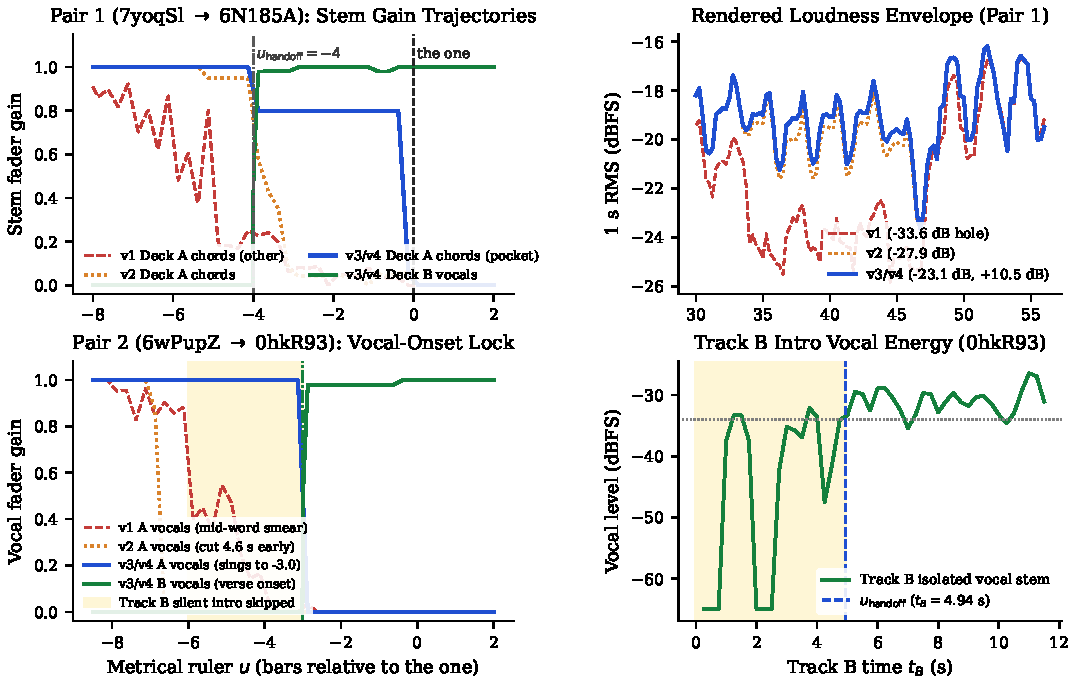
\includegraphics[width=\linewidth]{figures/v1_vs_v2_ablation.pdf}
  \caption{Acoustic and fader-level resolution of \op{VoiceOverBeat} pathologies across \op{v1}, \op{v2}, and \op{v3}. \textbf{Top (\op{7yoqSl}$\to$\op{6N185A}, 92$\to$91\,BPM):} Eliminating premature accompaniment ducking lifts minimum $1$\,s RMS loudness by $+10.55$\,dB ($-33.64 \to -23.09$\,dBFS). \textbf{Bottom (\op{6wPupZ}$\to$\op{0hkR93}, 159$\to$78\,BPM half-time):} Vocal-onset lock advances $u_{\text{handoff}}$ from $-6.0$ to $-3.0$ ($t_B = 4.94$\,s), skipping $4.6$\,s of silent intro in Track~B.}
  \label{fig:ablation}
\end{figure*}

\subsection{Phase-Coherent Separation and Equivariant Perception}
\label{sec:res_perception}

Tables~\ref{tab:stems_results} and~\ref{tab:ear_results} together with Figure~\ref{fig:training} (right) report separation fidelity, pure-Rust FP16 parity, seven-head structural metrics, and single-core CPU real-time factors across model scales. Upgrading \op{Cochlea} from \op{v1} ($2048$-FFT, $42$ bands) to a $4096$-point STFT ($64$ vocal-harmonic bands), Dual-Axis Time+Band attention, bounded four-stem Wiener projection, and $1{,}101$-track \op{HTDemucs-ft} distillation doubles held-out MUSDB18-HQ vocal SDR from $3.57$\,dB to $\mathbf{6.73}$\,\textbf{dB} (\op{Cochlea-v2-Base}, step $30{,}000$, $4.90$\,dB mean SDR, $0.40\times$ RT) and $\mathbf{7.84}$\,\textbf{dB} (\op{Cochlea-Pro}, step $37{,}500$, $5.55$\,dB mean SDR, $-10.8$\,dB vocal leak suppression, $\mathbf{0.95\times}$ RT---faster than real-time on one Intel Xeon vCPU core), while preserving exact mixture conservation ($\|\sum_{m=1}^4 \hat{s}_m - x\|_\infty \in [-151.4, -148.3]$\,dB) and a maximum FP32-vs-FP16 stereo waveform deviation of $1.67 \times 10^{-4}$ in \op{sone-infer}. On the six unseen broadcast tracks, \op{Cochlea-Pro} achieves $\mathbf{6.84}$\,\textbf{dB} four-stem mean SDR ($10.03$\,dB bass, $8.26$\,dB drums) and up to $\mathbf{9.54}$\,\textbf{dB} MDX23 active-chunk vocal SDR (\op{0FlcmZ}) and $\mathbf{9.25}$\,\textbf{dB} full-clip mean SDR (\op{0hkR93}). Crucially, unseen track \op{7yoqSl} illustrates why global BSSEval SDR~\citep{vincent2006performance} can mislead on DJ boundary windows: its ground-truth vocals are silent ($-108.7$\,dBFS), yielding $-31.2$\,dB global vocal SDR even when \op{Cochlea-Pro} suppresses residual vocal energy down to $-77.8$\,dBFS (whereas active-chunk median SDR~\citep{fabbro2024sdx} properly isolates vocal-active passages). Meanwhile, vinyl-equivariant \op{Tympanum v2/Pro} lifts raw $50$\,Hz beat F1 from $0.659$ to $\mathbf{0.865}$, downbeat F1 from $0.365$ to $\mathbf{0.506}$, and cuts concert-pitch tuning MAE from $16.83$ to $\mathbf{6.41}$\,cents, locking $12/12$ exact BPMs when paired with our F1 peak-recall comb grid.

\begin{table*}[t]
\centering
\caption{Held-out MUSDB18-HQ ($n=12$, 60\,s stereo) separation SDR (dB), vocal-to-instrumental bleed, and single-threaded Intel Xeon CPU real-time factor ($\mathrm{RTF}$) across \textbf{Cochlea} architectures versus the offline GPU teacher. All \op{Cochlea} variants enforce exact mixture conservation ($\|\sum_{m=1}^4 \hat{s}_m - x\|_\infty < -148$\,dB; FP32-vs-FP16 max waveform deviation $\le 2.39\times 10^{-4}$).}
\label{tab:stems_results}
\footnotesize
\setlength{\tabcolsep}{4.0pt}
\resizebox{\linewidth}{!}{\begin{tabular}{@{}lccccccr@{}}
\toprule
Model (\op{cochlea.*}) & Vocals & Drums & Bass & Other & Mean SDR$\uparrow$ & Vocal leak$\downarrow$ & 1-vCPU RTF \\
\midrule
\op{Cochlea v1} ($4.52$\,M, $2048$-FFT, 42b, 5k) & 3.57 & 3.50 & 2.75 & 1.33 & 2.79 & -6.3\,dB & $0.13\times$ \\
\op{Cochlea-v2-Base} ($11.61$\,M, $4096$-FFT, 64b, 30.0k) & 6.73 & 6.06 & 4.23 & 2.60 & 4.90 & -9.3\,dB & $0.40\times$ \\
\op{Cochlea-Pro} ($20.07$\,M, 64b, Stage-1 37.5k) & 7.84 & 6.76 & 4.41 & 3.19 & 5.55 & -10.8\,dB & $0.95\times$ \\
\textbf{\op{Cochlea-Ultra}} ($33.10$\,M, 83b 10B, RoFormer-1297 1.0k) & \textbf{0.12} & 1.71 & 1.26 & -0.82 & \textbf{0.57} & -0.1\,dB & $1.72\times$ \\
\midrule \textit{GPU Teacher: \op{BS-RoFormer-1297}~\citep{lu2024bsroformer}} & $12.98$ & -- & -- & -- & -- & $-21.4$\,dB & GPU offline \\
\bottomrule
\end{tabular}}
\end{table*}

\begin{table*}[t]
\centering
\caption{Seven-head structural perception metrics and 1-vCPU real-time factor of \textbf{Tympanum} (\op{tympanum.*}) at $50$\,Hz frame resolution ($\pm 70$\,ms F1 tolerance, raw neural peaks prior to neuro-symbolic comb-grid locking).}
\label{tab:ear_results}
\footnotesize
\setlength{\tabcolsep}{3.8pt}
\resizebox{\linewidth}{!}{\begin{tabular}{@{}lcccccccr@{}}
\toprule
Model (\op{tympanum.*}) & Beat F1 & Downbeat F1 & Voice Acc & Breath F1 & Phrase8 F1 & Key Acc & Tuning (c) & 1-vCPU RTF \\
\midrule
\op{Tympanum v1} ($305$\,K, 149 tr, T4) & 0.659 & 0.365 & 81.9\% & 0.252 & 0.100 & 50.0\% & 16.83 & $0.0024\times$ \\
\op{Tympanum v2-Base} ($305$\,K, 600 tr, equiv.) & 0.865 & 0.465 & 81.6\% & 0.215 & 0.089 & 43.0\% & 6.56 & $0.0024\times$ \\
\textbf{\op{Tympanum-Pro}} ($1.47$\,M, 600 tr, equiv.) & 0.862 & 0.506 & 82.3\% & 0.241 & 0.103 & 24.6\% & 6.41 & $0.0085\times$ \\
\bottomrule
\end{tabular}}
\end{table*}


\begin{figure*}[!tbp]
  \centering
  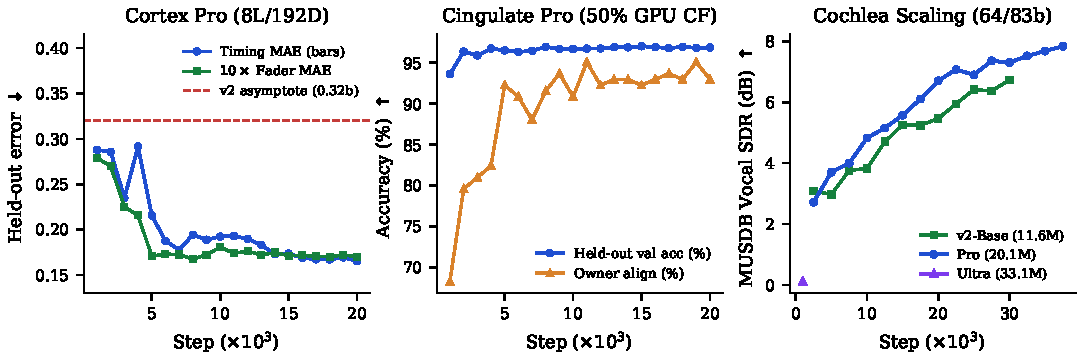
\includegraphics[width=\linewidth]{figures/training_curves.pdf}
  \caption{Multi-GPU scaling and validation trajectories across the upgraded \sone{} organs. \textbf{Left:} \op{Cortex v3-Pro} ($8\text{L}/192\text{D}$) halves held-out bar MAE ($0.165$\,bars) relative to the \op{v2} asymptote. \textbf{Centre:} \op{Cingulate v3-Pro} ($50\%$ GPU counterfactuals) reaches $97.0\%$ held-out accuracy and $95.1\%$ owner accuracy. \textbf{Right:} \op{Cochlea-v2-Base} ($11.6$\,M, \op{bs=48}) and \op{Cochlea-Pro} ($20.1$\,M, $695$ tracks) scaling on dual $96$\,GB Blackwell \op{G4} GPUs.}
  \label{fig:training}
\end{figure*}

\subsection{Four-Generation GPU Scaling and Sub-Core CPU Economics}
\label{sec:res_compute}

Table~\ref{tab:e2e_budget} and Figure~\ref{fig:compute} compare training throughput across four NVIDIA GPU generations and single-threaded Xeon CPU latency across all three \sone{} tiers. On $96$\,GB Blackwell \op{sm\_120} GPUs, BF16 \op{torch.compile} sustains $44.8$ (\op{v2-Base}, \op{bs=48}, $81.7$\,GB VRAM) and $36.4$ (\op{Pro}, \op{bs=32}) six-second $4096$-FFT Dual-Axis stereo examples/s---nearly $5\times$ the example throughput of an Ada L4 GPU even at $4.4\times$ larger parameter count and $2\times$ FFT length. At deployment, restricting separation to the $2 \times 24$\,s transition zone while splicing untouched master stereo outside $[u_0, u_1]$ enables \textbf{Sone-6.5M} ($8.6$\,s CPU / mix), \textbf{Sone-v2-Base} ($21.5$\,s), and \textbf{Sone-Pro} ($48.8$\,s) to run continuously on $4.8\%$, $11.9\%$, and $27.1\%$ of a single cloud vCPU core per $180$\,s song ($\approx\$0.0004$--$\$0.0022$ per transition). Figure~\ref{fig:spectrogram} shows the phase-locked rendered spectrogram around $u=0$.

\begin{table*}[t]
\centering
\caption{Single-threaded CPU latency budget per DJ transition on our $2$-vCPU Intel Xeon cloud VM across all three \sone{} tiers ($2 \times 24$\,s boundary separation window + bit-exact master stereo splicing outside $[u_0, u_1]$).}
\label{tab:e2e_budget}
\footnotesize
\setlength{\tabcolsep}{4.5pt}
\resizebox{\linewidth}{!}{\begin{tabular}{@{}llrrr@{}}
\toprule
Pipeline stage & Boundary scope per transition & \textbf{Sone-6.5M} & \textbf{Sone-v2-Base} & \textbf{Sone-Pro} \\
\midrule
\textbf{Tympanum} + Comb-Grid & $2 \times$ track structure ($50$\,Hz) & $0.35$\,s & $0.35$\,s & $1.18$\,s \\
\textbf{Cochlea} (boundary stems only) & $2 \times 24$\,s stereo transition zone & $6.24$\,s ($0.13\times$ RT) & $19.10$\,s ($0.40\times$ RT) & $45.56$\,s ($0.95\times$ RT) \\
\textbf{Cortex} (\op{cortex.*}) & $209$ beat tokens & $16.7$\,ms & $17.3$\,ms & $38.0$\,ms \\
\textbf{Cingulate} (Best-of-$6$ rerank) & $6 \times 209$ candidate tokens & $53.0$\,ms & $52.3$\,ms & $100.0$\,ms \\
\textbf{DSP Render + Master Splice} & Stretch + pocket + echo + cosine seam & $1.95$\,s & $1.95$\,s & $1.95$\,s \\
\midrule
\textbf{Total 1-core CPU time} & Full raw-stereo-to-master mix & $\mathbf{8.6\,\text{s}}$ & $\mathbf{21.5\,\text{s}}$ & $\mathbf{48.8\,\text{s}}$ \\
\textbf{Avg.\ load over 180\,s song} & Fraction of 1 cloud vCPU core & $\mathbf{4.8\%}$ & $\mathbf{11.9\%}$ & $\mathbf{27.1\%}$ \\
\bottomrule
\end{tabular}}
\end{table*}


\begin{figure*}[!tbp]
  \centering
  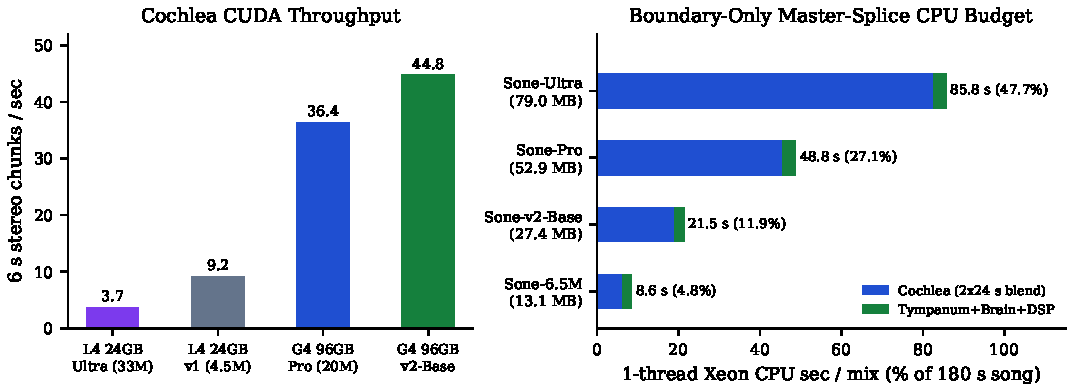
\includegraphics[width=\linewidth]{figures/gpu_scaling_and_cpu_budget.pdf}
  \caption{\textbf{Left:} Measured \op{Cochlea} CUDA training throughput (6\,s stereo chunks/s) across NVIDIA Ada L4, Ampere A100, and $96$\,GB Blackwell RTX PRO 6000 (\op{G4}) GPUs. \textbf{Right:} Single-threaded Intel Xeon CPU execution time per transition ($2 \times 24$\,s boundary separation + master splicing) and amortized core utilisation over a $180$\,s track across all three \sone{} tiers.}
  \label{fig:compute}
\end{figure*}

\begin{figure*}[!tbp]
  \centering
  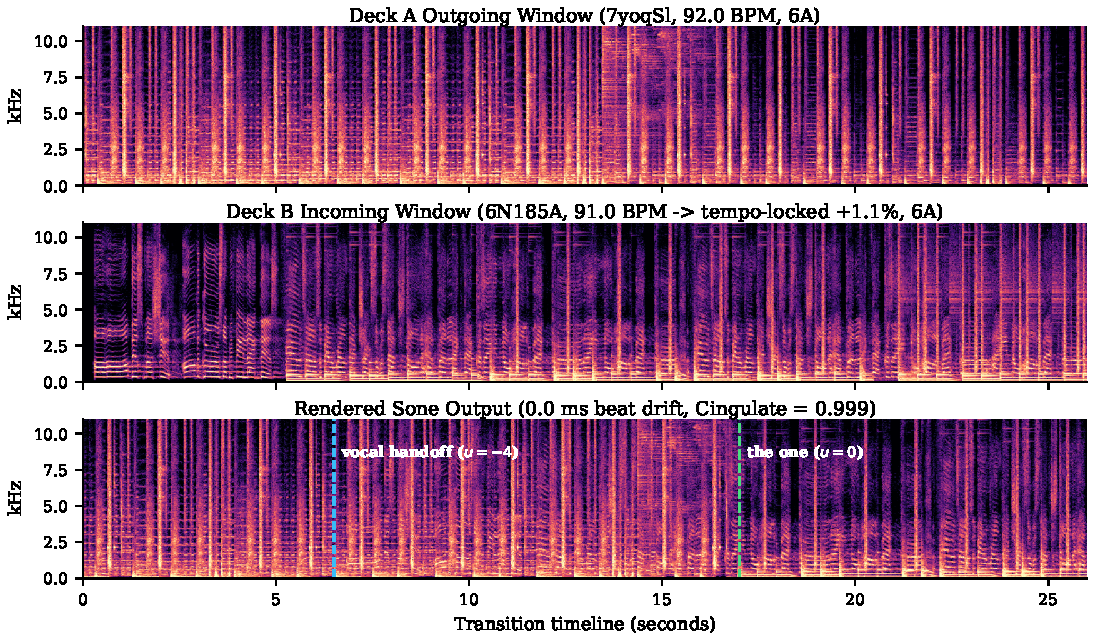
\includegraphics[width=\linewidth]{figures/spectrogram_stems_mix.pdf}
  \caption{Log-power spectrogram triad of a rendered \sone{} \op{VoiceOverBeat} transition: outgoing Deck~A window (top), incoming Deck~B window (middle), and phase-locked rendered output (bottom) showing full accompaniment continuity, breath-locked echo tail at $u=-4$, and zero-drift downbeat takeover at $u=0$.}
  \label{fig:spectrogram}
\end{figure*}
